\section{Konvexní funkce}\label{defKonv}

Nechť $f : D \subseteq \R^n \rightarrow \R$ a $C \subseteq D$ je neprázdná konvexní množina. \\
Řekněme, že $f$ je
\begin{enumerate}[(a)]
    \item konvexní na $C$, jestliže pro každé $x, y \in C$ a každé $\lambda \in [0,1]$ je
    \[
        f(\lambda x + (1-\lambda) y) \leq \lambda f(x) + (1-\lambda)f(y).
    \]
    \item ryze konvexní na $C$, jestliže pro každé dva různé body $x, y \in C$ a $\lambda \in (0,1)$ je
    \[
        f(\lambda x + (1-\lambda) y) < \lambda f(x) + (1-\lambda)f(y).
    \]
    \item konkávní (resp. ryze konkávní) na $C$, jestliže $(-f)$ je konvexní (resp. ryze konvexní) na $C$.
\end{enumerate}

\begin{multicols}{2}
    \begin{tikzpicture}[scale=2]
        \draw[->] (-2,0) -- (2,0);
        \draw[->] (0,-0.5) -- (0,3);

        \draw[thick, blue, domain=-1.5:1.5, smooth] plot (\x, {(\x)^2 + 0.5});

        \node at (1.2,2.3) [below right]{\small \textcolor{blue}{$f(x)$}};

        \draw[black!40!yellow, thick] (-1, 1.5) -- (0.5, 0.75);

        \draw[black!40!green, dashed] (-1,1.5) -- (-1, 0) node[below]{\small $x$};
        \fill[black!40!green] (-1, 1.5) circle(1pt) node[left]{\small $(x, f(x))$};

        \draw[black!40!red, dashed] (0.5,0.75) -- (0.5, 0) node[below]{\small $y$};
        \fill[black!40!red] (0.5, 0.75) circle(1pt) node[right]{\small $(y, f(y))$};

        \draw[yellow!40!red, dashed] (-0.25, 1/16 + 0.5) -- (-0.25, -0.05) node[below]{\small $C$};
        \fill[yellow!40!red] (-0.25, 1/16 + 0.5) circle(1pt) node[below left]{\small $B$};
        % \draw[yellow!40!red, <-] (-0.25 - 0.1, 1/16 + 0.5 + 0.03) -- (-0.75, 0.7) node[left]{\small $B$};

        \draw[yellow!40!red, dashed] (-0.25, 1/16 + 0.5) -- (-0.25, 1/16 + 1 + 1/16);
        \fill[yellow!40!red] (-0.25, 1/16 + 1 + 1/16) circle(1pt) node[below left]{\small $A$};
        % \draw[yellow!40!red, <-] (-0.25, 1/16 + 1 + 1/16 + 0.05) -- (-0.75, 1.7) node[left]{\small $A$};

    \end{tikzpicture}

\columnbreak

    \textcolor{yellow!40!red}{$A$} $= (\lambda x + (1-\lambda)y, \lambda f(x) + (1-\lambda)f(y))$\\
    \textcolor{yellow!40!red}{$B$} $= (\lambda x + (1-\lambda)y, f(\lambda x + (1-\lambda)y))$\\
    \textcolor{yellow!40!red}{$C$} $= \lambda x + (1-\lambda)y$

    Pozorování: \textcolor{black!40!yellow}{úsečka} vždy leží nad \textcolor{blue}{funkcí}.
\end{multicols}

\subsection{Příklad konvexní funkce}
Je afinní zobrazení $f : \R^n \rightarrow \R^n$ (tj. $f(x) = \langle x,a \rangle + b, b\in \R$) konvexní?

Důkaz.\\
Ať  $x, y \in \R^n, \lambda \in [0,1]$.
\begin{align*}
    f(\lambda x + (1-\lambda) y) &= \langle \lambda x + (1-\lambda) y, a\rangle + b\\
    &= \lambda \langle x, a\rangle + (1-\lambda) \langle y, a\rangle + \lambda b + (1-\lambda)b\\
    &= \lambda f(x) + (1-\lambda) f(y) \implies f \text{ je konvexní i konkávní.} \qed
\end{align*}

\subsection{Příklad konvexní funkce}
Je funkce $f(x) = \| x\|$ konvexní?

Důkaz.\\
Ať $x, y \in \R^n, \lambda \in [0,1]$.
\begin{align*}
    f(\lambda x + (1-\lambda) y) &= \| \lambda x + (1-\lambda)y\| \stackrel{\text{odhad}}{\leq} \| \lambda x\| +
    \| (1-\lambda) y\| = \lambda \| x\| + (1-\lambda) \| y\| \\
    &= \lambda f(x) + (1-\lambda) f(y) \implies f \text{ je konvexní.} \qed
\end{align*}

\subsection{Dolní úrovňová množina}
Dolní úrovňová množina funkce $f : D \subseteq \R^n \rightarrow \R^n$ hladiny $\alpha \in \R$ je množina
\[
    \lev_{\leq} (f; \alpha) \coloneq \bc{x \in D \mid f(x) \leq \alpha}.
\]
Je-li $f$ konvexní na $C \subseteq \R^n$, pak $\lev_{\leq} (\restr{f}{C}; \alpha)$ je konvexní pro
$\forall \alpha \in \R$.
\begin{figure}[H]
    \centering
    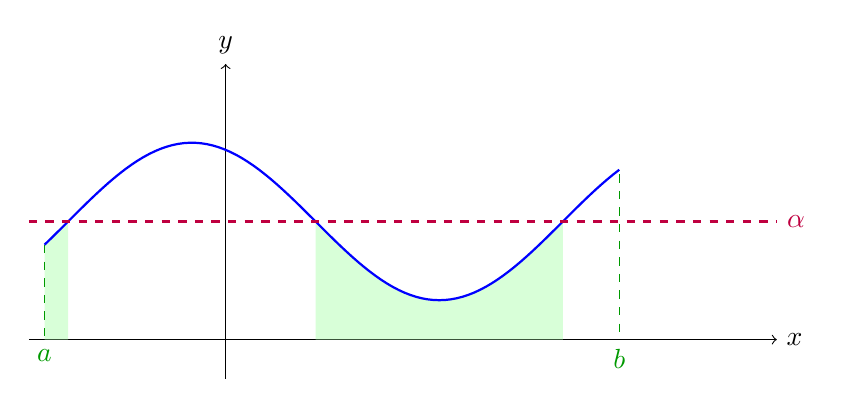
\begin{tikzpicture}[domain=-0.3:7, samples=100]
        \draw[->] (-2.5,0) -- (7,0) node[right] {$x$};
        \draw[->] (0,-0.5) -- (0,3.5) node[above] {$y$};

        % Segment I: x in [-2.3, -2]
        \fill[green!30, opacity=0.5]
        plot[domain=-2.3:-2, samples=50] (\x, {sin((\x+2) r)+1.5})
        -- (-2,0) -- (-2.3,0) -- cycle;

        % % Segment II: x in [-2, pi-2]
        % \fill[green!30, opacity=0.5]
        % (-2,1.5) -- ({pi-2},1.5) -- ({pi-2},0) -- (-2,0) -- cycle;

        % Segment III: x in [pi-2, 2*pi-2]
        \fill[green!30, opacity=0.5]
        plot[domain={pi-2}:{2*pi-2}, samples=50] (\x, {sin((\x+2) r)+1.5})
        -- ({2*pi-2},0) -- ({pi-2},0) -- cycle;

        % % Segment IV: x in [2*pi-2, 5]
        % \fill[green!30, opacity=0.5]
        % ({2*pi-2},1.5) -- (5,1.5) -- (5,0) -- ({2*pi-2},0) -- cycle;

        \draw[blue, thick] plot ({\x-2}, {sin(\x r) + 1.5});

        \draw[purple, thick, dashed] (-2.5, 1.5) -- (7, 1.5) node[right]{$\alpha$};

        \draw[black!40!green, dashed] (-2.3, 1.2) -- (-2.3, 0) node[below]{$a$};
        \draw[black!40!green, dashed] (5, 2.1) -- (5, 0) node[below]{$b$};
    \end{tikzpicture}
\end{figure}
Důkaz.

Ať $x, y \in \lev_{\leq}(\restr{f}{C}; \alpha), \lambda \in [0,1]$.\\
Cíl: $\lambda x + (1-y)\lambda \stackrel{?}{\in} \lev_{\leq} (\restr{f}{C}; y)$.
\[
    f(\lambda x + (1-\lambda)y) \leq \lambda f(x) + (1-\lambda) f(y) \leq \lambda \alpha + (1-\lambda) \alpha = \alpha.
    \qed
\]

Poznámka.

Opačná implikace neplatí. Tedy pomocí dolní úrovňové množiny \textbf{nelze} určit, jestli původní funkce je konvexní.

Například $f = x^3$ není konvexní funkce na intervalu $x = [-2, 2]$, ale když zvolíme $\alpha = 8$, tak dolní úrovňová
množina bude konvexní. % TODO: nákres

\subsection{Použití dolní úrovňové množiny}
Je množina $M = \bc{x \in \R^2 \mid \| x\| \leq 1, \left\langle x,
\begin{pmatrix}
    2 \\
    1
\end{pmatrix}
\right\rangle \leq 1}$ konvexní?

Důkaz.

Rozdělme si množinu $M$ na dvě podmnožiny $M_1$ a $M_2$, kde:

$M_1 = \bc{x \in \R^2 \mid \| x\| \leq 1} = \lev_{\leq} (\| x\|, 1) \rightarrow$ konvexní, protože norma je konvexní
funkce.

$M_2 = \bc{x \in \R^2 \mid \left\langle x,
\begin{pmatrix}
    2 \\
    1
\end{pmatrix}
\right\rangle \leq 1} = \lev_{\leq} \left(\left\langle x,
\begin{pmatrix}
    2 \\
    1
\end{pmatrix}
\right\rangle, 1\right) \rightarrow$ konvexní, protože skalární součin je konvexní.

To nám ale dává průnik dvou konvexních množin, tedy $M = M_1 \cap M_2$ je také konvexní. $\qed$

% TODO: nákres
\newpage
\subsection{Součet a součin zachovávají konvexitu}\label{ssKonv}
Mějme funkce $f, g$, které jsou konvexní na $C$, $\alpha \geq 0$. Pak:
\begin{enumerate}[(a)]
    \item $f+g$ je konvexní na $C$
    \item $\alpha f$ je konvexní na $C$
\end{enumerate}
Důkaz.

(a) Ať $\lambda \in [0,1], x, y \in C$.
\[
    (f+g)(\lambda x + (1-\lambda)y) = \underbrace{f(\lambda x + (1-\lambda)y)}_{\leq \lambda f(x) + (1-\lambda)f(y)} +
    \underbrace{g(\lambda x + (1-\lambda)y)}_{\leq \lambda g(x) + (1-\lambda)g(y)}
\]
\[
    \leq \lambda f(x) + (1-\lambda)f(y) + \lambda g(x) + (1-\lambda)g(y) = \lambda (f+g)(x) + (1-\lambda)(f+g)(y). \qed
\]

(b) Ať $\lambda \in [0,1], x, y \in C, \alpha \geq 0$.
\[
    \alpha f(\lambda x + (1-\lambda)y) \leq \alpha f(\lambda x) + \alpha f((1-\lambda)y) = \alpha \lambda f(x) + 
    \alpha (1-\lambda)f(y). \qed
\]

\subsection{Příklad ověření konvexity}
Je funkce $f(x) = e^x - 3 \ln x + 2x$ konvexní?

Rozeberme si jednotlivé části funkce.
\begin{itemize}
    \item $e^x$ $\dots$ exponenciála je z grafu očividně konvexní.
    \item $-3 \ln x$ $\dots$ logaritmus je konkávní, ale díky \enquote{$\minus$} se celý výraz stane konvexní. Násobení
    konstatou konvexitu neovlivní, viz důkaz \hyperref[ssKonv]{(b)}.
    \item $2x$ $\dots$ lineární funkce je konvexní.
\end{itemize}
Protože všechny komponenty funkce $f$ jsou konvexní, pak je i funkce $f$ nutně konvexní.

\subsection{Skládání zachovává konvexitu}
Skládání konvexních funkcí není obecně konvexní funkce. Například: $f(x) = x^2$ a $g(x) = x^2 -1$ jsou konvexní, ale
\[
    (f \circ g)(x) = (f(g(x))) = (x^2 - 1)^2 \text{ z grafu očividně není konvexní.}
\]

1. Mějme tedy tvrzení.

Nechť $f$ je konvexní na $K \subseteq \R^m$, $C \subseteq \R^n$ je neprázdná konvexní a $g : \R^n \rightarrow \R^m$ je
afinní. Jestliže $g(C) \subseteq K$ (tedy $g$ \enquote{obtiskne} množinu $C$ do $K$), pak $f \circ g$ je konvexní na
$C$. \label{skladFun}

Důkaz.\\
Ať $x, y \in C$, $\lambda \in [0,1]$.\\
Pak
\[
    f(g(\lambda x + (1-\lambda)y))
    \stackrel{g \text{ je \hyperref[sec:afin]{afinní}}}{=} f(\lambda \overbrace{g(x)}^{\in K}
    + (1-\lambda) \overbrace{g(y)}^{\in K})
    \stackrel{f \text{ je \hyperref[defKonv]{konvexní}}}{\leq} \lambda f((g(x))) + (1-\lambda) f(g(y))
\]
A to přesně dle \hyperref[defKonv]{definice konvexní} funkce dává, že $f \circ g$ je konvexní funkce. $\qed$

2. Mějme ještě druhé tvrzení.

Jestliže $f$ je konvexní a \textbf{neklesající} na intervalu $I$, $g$ je konvexní na $C \subseteq \R^n$ a
$g(C) \subseteq I$, pak $f \circ g$ je konvexní na $C$.

Důkaz.\\
Ať $x, y \in C$, $\lambda \in [0,1]$.\\
Pak
\[
    f(\underbrace{g(\lambda x + (1-\lambda)y)}_{\substack{\leq \lambda g(x) + (1-\lambda)g(y) \\ \text{odhad, díky
    konvexitě }g }}) \underset{g \text{ je konvexní}}{\overset{f \text{ je neklesající}}{\leq}} f(\lambda g(x) +
    (1- \lambda) g(y)) \overset{f \text{ je \hyperref[defKonv]{konvexní}}}{\leq} \lambda f(g(x)) + (1-\lambda) f(g(y))
\]
A to přesně dle \hyperref[defKonv]{definice konvexní} funkce dává, že $f \circ g$ je konvexní funkce. $\qed$

\subsection{Věta o extrémech konvexních funkcí}
Nechť $f$ je konvexní na $C \subseteq \R^n$. Potom platí:
\begin{enumerate}[(a)]
    \item Každý bod lokálního minima $f$ na $C$ je bodem minima $f$ na $C$.
    \item Množina $\argmin_{x \in C} f(x)$ je konvexní. Je-li navíc $f$ ryze konvexní na $C$, pak existuje nejvýše jeden
    bod minima funkce $f$ na $C$.
\end{enumerate}

Důkaz (a).\\
Sporem. Ať $\hat x \in C$ je bod lokálního minima $f$ na $C$ a ať existuje $\hat y \in C$ tak, že
$f(\hat y) < f(\hat x)$. $\lambda \in [0,1)$.\\
Pak
\[
    f(\lambda \hat x + (1-\lambda) \hat y) \overset{f \text{ je \hyperref[defKonv]{konvexní}}}{\leq}
    \lambda f(\hat x) + (1-\lambda) \overbrace{f(\hat y)}^{< f(\hat x)} \underset{\text{odhad}}{<}
    \lambda f(\hat x) + (1-\lambda) f(\hat x) = f(\hat x)
\]
Což je ale spor s naším předpokladem, protože kdykoliv si vezmu bod na úsečce mezi $\hat x$ a $\hat y$, tak je v něm
hodnota ostře menší než funkční hodnota v bodě $f(\hat x)$. $\qed$

Důkaz (b).\\
Ať $\hat x, \hat y \in \argmin_{x \in C} f(x)$, $\lambda \in [0,1]$.\\
Pak
\[
    f(\lambda \hat x + (1-\lambda) \hat y) \overset{f \text{ je \hyperref[defKonv]{konvexní}}}\leq \lambda f(\hat x) +
    (1-\lambda) \overbrace{f(\hat y)}^{= f(\hat x)} = f(\hat x)
\]
$\implies \lambda \hat x + (1-\lambda) \hat y \in \argmin_{x \in C} f(x)$. $\qed$

Ať $f$ je navíc ryze konvexní na $C$.\\
Cíl: $\argmin_{x \in C} f(x)$ má nejvýše jeden prvek.

Důkaz.\\
Sporem. Ať $\hat x, \hat y \in \argmin_{x \in C} f(x)$, $\hat x \not=\hat y$. $\lambda \in (0,1)$.\\
Pak
\[
    f(\lambda \hat x  + (1-\lambda) \hat y) \overset{f \text{ je ryze konv.}}{<} \lambda f(\hat x) + (1-\lambda)
    \underbrace{f(\hat y)}_{= f(\hat x)} = f(\hat x)
\]
Což je ale spor, protože mám nějakou funkční hodnotu bodu úsečky mezi $\hat x$ a $\hat y$ ostře menší jak funkční
hodnotu bodu $\hat x$. To ale nemůže nastat, protože jako body minima funkce $f$ na $C$ musí mít stejnou hodnotu. Body
$\hat x$ a $\hat y$ musí tedy nutně být stejné body. $\qed$

\subsection{Věta o konvexitě a první derivaci}\label{konvDeriv} % TODO: graf
Nechť $\Omega \subseteq \R^n$ je otevřená, $C \subseteq \Omega$ neprázdná konvexní a $f \in C^{1} (\Omega)$. Potom
platí:
\begin{enumerate}[(a)]
    \item $f$ je konvexní na $C$ právě tehdy, když pro každé $x, y \in C$ je
    \[
        f(x) + \langle \nabla f(x), y-x\rangle \leq f(y).
    \]
    \item $f$ je ryze konvexní na $C$ právě tehdy, když pro každé dva různé body $x, y \in C$ je
    \[
        f(x) + \langle \nabla f(x), y-x\rangle < f(y).
    \]
\end{enumerate}
Důkaz (b) vynecháme.

Důkaz (a).

\enquote{$\Rightarrow$}: Ať $x, y \in C$, $\lambda \in (0,1]$.
\[
    f(x + \lambda (y-x)) = f(\lambda y + (1-\lambda)x) \overset{f \text{ je \hyperref[defKonv]{konvexní}}}{\leq}
    \lambda f(y) + (1 - \lambda)f(x) = f(x) + \lambda [f(y) - f(x)]
\]
\[
    \Rightarrow \underbrace {\frac {f(x + \lambda (y-x)) - f(x)}{\lambda}}_{\substack{{ = \langle \nabla f(x),
    y-x\rangle \text{ pro } \lambda \rightarrow 0_+}\\{\text{z definice směrové derivace}}}} \leq f(y) - f(x). \qed
\]
\enquote{$\Leftarrow$}: Ať $x, y \in C$, $\lambda \in [0,1]$.

$z \coloneq \lambda x + (1-\lambda) y \in C$\\
Z předpokladu:
\begin{align*}
    & f(z) + \langle \nabla f(z), x - z\rangle \leq f(x) \quad / \cdot \lambda \\
    & f(z) + \langle \nabla f(z), y - z\rangle \leq f(y) \quad / \cdot (- \lambda)
\end{align*}
Pronásobením a sečtením dostaneme:
\[
    f(z) + \lambda \langle \nabla f(z), \underbrace{\lambda x + (1-\lambda)y}_{z} - z\rangle \leq \lambda f(x) +
    (1-\lambda)f(y)
\]
\[
    \Rightarrow f(z) \leq \lambda f(x) + (1-\lambda)f(y)
\]
Což ale po dosazení za $z$ je přesně ta nerovnost, která říká, že $f$ je konvexní. $\qed$

\subsection{Věta o konvexitě a druhé derivaci}\label{konvDDeriv}
Nechť $\Omega \subseteq \R^n$ je otevřená, $C \subseteq \Omega$ neprázdná konvexní a $f \in C^{2} (\Omega)$. Potom platí:
\begin{enumerate}[(a)]
    \item Jestliže pro každé $x \in C$ je $\nabla^2 f(x)$ positivně semidefinitní matice, pak $f$ je konvexní na C.
    \item Jestliže $f$ je konvexní na $C$ a $C$ je otevřená, potom $\nabla^2 f(x)$ je positivně semidefinitní matice pro
    každé $x \in C$.
    \item Jestliže pro každé $x \in C$ je $\nabla^2 f(x)$ positivně definitní matice, pak $f$ je ryze konvexní na $C$.
\end{enumerate}

\newpage
Důkaz (a).

Ať $x, y \in C$.

Taylorův polynom: existuje $\xi \in \bc{\lambda x + (1-\lambda)y \mid \lambda \in (0,1)} \subseteq C$ tak, že
\[
    f(y) = f(x) + \langle \nabla f(x), y-x\rangle + \underbrace{\frac{1}{2} \left\langle \nabla^2 f(\xi) (y-x),
    y-x\right\rangle}_{\geq 0}
\]
\[
    \Rightarrow f(y) \geq f(x) + \langle \nabla f(x), y-x\rangle
\]
Což je přesné znění \hyperref[konvDeriv]{věty o konvexitě a první derivaci}. Tedy $f$ je nutně konvexní na $C$.
\\
Důkaz (b).

Cíl: $\langle \nabla^2 f(x)y, y\rangle \geq 0$, $\forall y \in \R^n$

Ať $x \in C, y \in \R^n$.

Pak
$C$ otevřená $\Rightarrow$ existuje $\delta > 0$ tak, že $x + \alpha y \in C$ $\forall \alpha \in (0, \delta]$.

Taylorův polynom:
\[
    f(x+ \alpha y) = f(x) + \alpha \langle \nabla f(x), y\rangle + \frac{1}{2}\alpha^2 \langle \nabla^2 f(x)y, y\rangle
    + \alpha^2 \| y\|^2 \omega(\alpha y),
\]
kde $w$ má nulovou limitu v $0$.

Použijme fakt, že $f$ je konvexní:
\[
    f(x+\alpha y) \geq f(x) + \langle \nabla f(x), \alpha y\rangle
\]
Když tedy dosadíme:
\[
    f(x) + \alpha \langle \nabla f(x), y\rangle + \frac{1}{2}\alpha^2 \langle \nabla^2 f(x)y, y\rangle
    + \alpha^2 \| y\|^2 \omega(\alpha y) \geq f(x) + \langle \nabla f(x), \alpha y\rangle
\]
Upravíme a podělíme výrazem $\frac{1}{2}\alpha^2$ ($\alpha > 0$).
\[
   \langle \nabla^2 f(x)y, y\rangle + \underbrace{2 \| y\|^2 \omega(\alpha y)}_{\rightarrow 0 \text{ pro }
   \alpha \rightarrow 0_+} \geq 0
\]
V limitě $\alpha \rightarrow 0_+$ tedy máme $\langle \nabla^2 f(x)y, y\rangle \geq 0$, což je přesně to, co jsme chtěli.
$\qed$

Poznámka. Nutnost otevřenosti $C$ je velmi důležitá!

Důkaz (c). Podobně jako (a).

\subsection{Příklad ověření konvexnosti pomocí derivace}
$f(x, y) = x^2 - y^2$ je konvexní na $\R \times \bc{0}$. ($\rightarrow$ množina $\R \times \bc{0}$ není
otevřená, jedná se o přímku)

$\nabla^2 f(x, y) =
\begin{bmatrix}
    2 & \phantom{-}0 \\
    0 & -2
\end{bmatrix}$ je indefinitní, tedy funkce $f(x, y)$ není konvexní.

\subsection{Příklad ověření konvexnosti pomocí derivace}
$f(x, y) = x^2 + xy + y^2$ je ryze konvexní.

$\nabla^2 f(x, y) =
\begin{bmatrix}
    2 & 1 \\
    1 & 2
\end{bmatrix}$ $\rightarrow$ $2>0$, $\det \nabla^2 f(x,y) = 4-1>0$ $\implies$ dle Sylvesterova kritéria je
$\nabla^2 f(x,y)$ positivně definitní.

A podle bodu (c) \hyperref[konvDDeriv]{věty o konvexitě a druhé derivaci} můžeme říct, že funkce $f$ je ryze konvexní.
\newpage
\subsection{Příklad ověření konvexnosti funkce s parametrem}
Mějme funkci $f(x) = \langle Ax, x\rangle$, kde
\[
A = \begin{bmatrix}
    2 & 2 & 3 \\
    1 & 3 & 1 \\
    1 & 2 & \alpha
\end{bmatrix}, \alpha \in \R \text{ je parametr.}
\]
Pro jaké $\alpha$ je funkce $f$ konvexní?
\[
    \nabla^2 f(x) = \overbrace{A + A^T}^{\text{ze symetrie}} =
    \begin{bmatrix}
        4 & 3 & 4 \\
        3 & 6 & 3 \\
        4 & 3 & 2 \alpha
    \end{bmatrix}
\]
\[
    \det \nabla^2 f(x) =
    \begin{vmatrix}
        4 & 3 & 4 \\
        3 & 6 & 3 \\
        4 & 3 & 2 \alpha
    \end{vmatrix} \underset{R_3 - R_1}{=}
    \begin{vmatrix}
        4 & 3 & 4 \\
        3 & 6 & 3 \\
        0 & 0 & 2 \alpha - 4
    \end{vmatrix} = (2 \alpha - 4)
    \begin{vmatrix}
        4 & 3 \\
        3 & 6
    \end{vmatrix} = 3 (2 \alpha - 4)
    \begin{vmatrix}
        4 & 3 \\
        1 & 2
    \end{vmatrix} = 30 (\alpha - 2)
\]
Tedy aby $f$ byla konvexní funkce: $30 (\alpha - 2) \geq 0 \iff \alpha \geq 2$.

Musíme vyšetřit menší minory matice.

Vyškrtněme 3. řádek a 3. sloupec:
\[
    \begin{vmatrix}
        4 & 3 \\
        3 & 6
    \end{vmatrix} = 15 > 0
\]
Vyškrtněme 2. řádek a 2. sloupec:
\[
    \begin{vmatrix}
        4 & 4 \\
        4 & 2 \alpha
    \end{vmatrix} = 8
    \begin{vmatrix}
        1 & 1 \\
        2 & \alpha
    \end{vmatrix} = 8 (\alpha -2) \geq 0 \iff \alpha \geq 2 \dots \text{tuto podmínku již vyžadujeme.}
\]
Vyškrtněme 1. řádek a 1. sloupec:
\[
    \begin{vmatrix}
        6 & 3 \\
        3 & 2 \alpha
    \end{vmatrix} = 3
    \begin{vmatrix}
        2 & 1 \\
        3 & 2\alpha
    \end{vmatrix} = 3 (4\alpha -3) \geq 0 \iff \alpha \geq \frac{3}{4} \dots \text{vyžadujeme již silnější podmínku.}
\]
A teď zbylé minoru po vyškrtání dvou řádků a sloupců:
\[
    4 \geq 0, \quad 6 \geq 0, \quad 2 \alpha \geq 0 \iff \alpha \geq 0 \dots \text{vyžadujeme již silnější podmínku.}
\]

$\implies$ Pokud $\alpha \geq 2$, pak je funkce $f$ konvexní. Při $\alpha > 2$ je ryze konvexní.

\subsection{Příklad ověření konvexity množiny}
Mějme množinu
\[
    M = \bc{
        \begin{bmatrix}
            x \\
            y
        \end{bmatrix} \in \R^2 \, \middle| \, x + 2e^{-x+y^2} \leq 4, \, -x^2 + 3xy - 3y^2 \geq -1
    }.
\]
Je $M$ konvexní?

\begin{flalign*}
    \text{Označme:} \quad &g_1(x, y) = x + 2 e^{-x+y^2} \dots M_1 = \bc{
        \begin{bmatrix}
            x \\
            y
        \end{bmatrix} \, \middle| \, g_1 (x, y) \leq 4}& \\
        &g_2(x, y) = x^2 -3xy + 3y^2 \dots M_2 = \bc{
            \begin{bmatrix}
                x \\
                y
            \end{bmatrix} \, \middle| \, g_2 (x, y) \leq 1}
\end{flalign*}
$M = M_1 \cap M_2 \implies$ ukážeme konvexnost $M_1$ a $M_2$, protože průnik zachovává konvexitu.\\
$\implies g_1$ a $g_2$ musí být konvexní.

\begin{itemize}
    \item $g_1$:
        \begin{itemize}
            \item $x$ je afinní funkce $\rightarrow$ konvexní.
            \item součet zachovává konvexitu.
            \item násobení zachovává konvexitu.
            \item exponenciála je konvexní funkce (dokonce striktně rostoucí).
            \item vnitřní funkce ($-x + y^2$) je také konvexní.
        \end{itemize}
        $\implies g_1$ je konvexní funkce $\implies M_1$ je konvexní množina.
    \item $g_2$:
        \begin{itemize}
            \item kvadrát je konvexní.
            \item je ale člen \enquote{$xy$} konvexní? Musíme se podívat na Hessovu matici.
        \end{itemize}
\end{itemize}
\[
    \nabla^2 g_2(x, y) =
    \begin{bmatrix}
        \phantom{-}2 & -3 \\
        -3 & \phantom{-}6
    \end{bmatrix}
\]
\[
    \begin{rcases*}
        \det \nabla^2 g_2(x, y) = 12 - 9 = 3 > 0 \\
        2 \geq 0
    \end{rcases*} g_2 \text{ je (ryze) konvexní funkce } \implies M_2 \text{ je konvexní množina.}
\]
Protože $M_1$ i $M_2$ jsou konvexní množiny, pak nutně i $M_1 \cap M_2 = M$ je konvexní množina.
